Aufgrund der De Broglie-Wellenlänge haben auch Elektronen eine Wellenlänge, wenn sie einen Impuls besitzen, also bewegt sind.

Nun gilt es, Interferenzerscheinungen zu zeigen, was die Theorie beweisen würde, da es Wellencharakteristika zeigen würde.

\subsection{Theoretische Bestimmung der Wellenlänge}

Theoretisch lässt sich die De-Broglie-Wellenlänge $\lambda$ durch das Gleichsetzen der Gleichung des Impulses $\vec{p}=m\cdot\vec{v}$ mit der Formel für den Photonenimpuls $\vec{p}=\frac{h}{\lambda}$ berechnen:

\begin{align}	\label{eq:LambdaTheorie}
\begin{split}
	m_e \cdot v &= \frac{h}{\lambda} \\
	\lambda &= \frac{h}{m_e \cdot v}
\end{split}
\end{align}

Um die Geschwindigkeit $v$ bei einem Versuch mit Elektronenbeschleunigung durch ein elektrisches Feld zu ersetzen, setzt man die Gleichungen der kinetischen Energie $E_{kin}$ mit der Gleichung der Elektrischen $E_{el}$ gleich und formt anschließend nach $v$ um (Siehe: \referenz{sec:BraunscheRoehre}):

\begin{align}
\begin{split}
	v = \sqrt{\frac{2q_e \cdot U_B}{m_e}}
\end{split}
\end{align}

\noindent Durch Einsetzen in Gleichung \ref{eq:LambdaTheorie} folgt dann die theoretische Wellenlänge des Elektrons, die aus dem Versuchsaufbau zu erwarten ist:

\begin{align}
\begin{split}
	\lambda &= \frac{h \sqrt{m_e}}{m_e \cdot \sqrt{2q_e \cdot U_B}} \\
	\lambda &= \frac{h}{\sqrt{m_e} \cdot \sqrt{2q_e \cdot U_B}}
\end{split}
\end{align}


\subsection{Interferenz an Graphit}

Da Elektronen der Theorie nach eine sehr kleine Wellenlänge haben, benutzt man Kristalle, um Interferenzmuster zu erzeugen. An den Netzebenen des Kristalls, in denen die Atome regelmäßig angeordnet sind, werden Elektronen gestreut, ähnlich wie Licht an dünnen Schichten (Siehe: \referenz{sec:interferenz_schicht}). Auf dem Leuchtschirm der Röhre kommt es je nach Gangunterschied über die verschiedenen Netzebenen zu Maxima und Minima.

\begin{Wichtig}
	Bei Grafit haben die Atome in einer Ebene einen anderen Abstand $d$ zu einander, als die Atome zwischen den Ebenen. Es gibt also zwei \glqq Spaltabstände\grqq{} und folglich auch zwei Maxima 1. (2., $\cdots$, n.) Ordnung.
\end{Wichtig}

\begin{figure}[h!]
	\centering 
	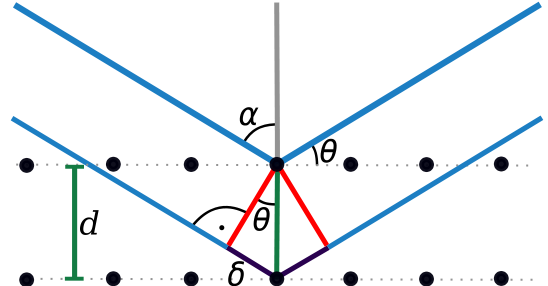
\includegraphics[width=0.7\textwidth]{Streuung_an_Graphit}
	\caption{Darstellungen der Beziehungen. Achtung: $\alpha$ ist hier mit $\Theta$ vertauscht!}
	\label{fig:e-angrafit}
\end{figure}

Der Gangunterschied $\delta$, siehe Zeichnung\endnote{\glqq Bragg\grqq{} by Dipl.-Phys. (JPG-version), Matthias M. (SVG-version) - /home/matthias/Desktop. Licensed under Public Domain via Wikimedia Commons - \url{https://commons.wikimedia.org/wiki/File:Bragg.svg}}, ist $\delta = 2d \cdot \sin{\alpha}$ und für konstruktive Interferenz, also ein Maximum, muss er ein natürliches Vielfaches der Wellenlänge $\lambda$ sein:

\begin{align}
\begin{split}
	n \cdot \lambda = 2d \cdot \sin{\alpha}
\end{split}
\end{align}

\noindent Daraus folgt die Bragg'sche Bedingung:

\begin{align}
\begin{split}
	\sin{\alpha} = \frac{n \cdot \lambda}{2d}
\end{split}
\end{align}


\subsubsection{Versuch}

Im Versuch wird ein beschleunigter Elektronenstrahl auf einen Graphitkristall geleitet. An diesem kommt es zur Streuung und es bilden sich zwei ringförmige Maxima auf dem Schirm, welcher so beschichtet ist, dass er unter Elektronenstimulation leuchtet.

Bezeichnet man den Abstand vom Maximum $n.$ Ordnung zum Maximum $0.$ Ordnung mit $r$ und den Abstand vom Kristall zum Schirm mit $a$ folgt gemäß Winkelbeziehungen:

\begin{align}
	\tan{2\alpha} = \frac{r}{a}
\end{align}

Um die Wellenlänge der Elektronen nun experimentell zu bestimmen, setzt man diese Formel mit der Bragg'schen Gleichung gleich. Man kann folgende Kleinwinkelnäherung für $\alpha > 10\degree$ anwenden:

\begin{align}
\begin{split}
	2\sin{\alpha} = tan{2\alpha}
\end{split}
\end{align}

\noindent Dann folgt:

\begin{align}
\begin{split}
	\frac{n\cdot\lambda}{2d} &= \frac{r}{a} \\
	\lambda &= \frac{2dr}{n\cdot l}
\end{split}
\end{align}

\noindent \textbf{Hiermit hat man eine Gleichung in der nur messbare Werte stecken und kann das Ergebnis mit dem theoretischen Ergebnis von oben vergleichen.}

\paragraph{Ohne Winkelnäherung}

\begin{align}
\begin{split}
	2\cdot\arcsin(\frac{n\cdot \lambda}{2d}) &= \arctan(\frac{r}{l})  \\
	\arcsin(\frac{n\cdot \lambda}{2d}) &= \frac{1}{2}\cdot\arctan(\frac{r}{l}) \\
	\frac{n\cdot \lambda}{2d} &= \sin(\frac{1}{2}\cdot\arctan(\frac{r}{l})) \\
	\lambda &= \sin(\frac{1}{2}\cdot\arctan(\frac{r}{l}))\cdot \frac{2d}{n}
\end{split}
\end{align}

\begin{NiceToKnow}
Es kommt nur zur Interferenz, wenn die Bragg'sche Gleichung erfüllt ist. Dafür muss $\alpha$, für eine bestimmte Wellenlänge, auch eine bestimmte Größe haben. Im Experiment wird deshalb eine Graphitfolie benutzt, auf der die Kristallgitter in den verschiedensten Anordnungen liegen. So ist statistisch gesehen immer ein Kristall im richtigen Winkel zum Elektronenstrahl.
\end{NiceToKnow}


\subsection{Interferenz am Doppelstpalt}

Grundsätzlich gelten die gleichen Formeln wie bei der Interferenz mit Licht (Siehe \referenz{sec:interferenz_spalt}). Allerdings muss der Spaltabstand $d$, aufgrund der sehr kleinen Wellenlängen, ebenfalls sehr klein sein, damit man überhaupt ein Interferenzmuster detektieren kann. Auch wenn man dies berücksichtigt, ist das Interferenzmuster trotzdem so klein, dass man es nur mit einem Elektronenmikroskop sichtbar machen kann.

Bedingungen für konstruktive Interferenz: $\delta = n \cdot \lambda$; für destruktive Interferenz: $\delta = (n-\frac{1}{2}) \cdot \lambda$.


\subsubsection{Versuch}

Um die Wellenlänge $\lambda$ experimentell herauszufinden, gilt, wenn $d$ der Spaltabstand ist, $a$ der Abstand zum Schirm und $d_k$ der Abstand des k. Maximum zum 0. Maximum, ist:

\begin{align}
\begin{split}
	\tan{\alpha} = \frac{d_k}{a}
\end{split}
\end{align}

\noindent und:

\begin{align}
\begin{split}
	\sin{\alpha} = \frac{k \cdot\lambda}{d}
\end{split}
\end{align}

\noindent Dann entweder durch Kleinwinkelnäherung:

\begin{align}
\begin{split}
	\lambda = \frac{d_k \cdot d}{k \cdot a}
\end{split}
\end{align}

\noindent oder ohne:

\begin{align}
\begin{split}
	\lambda = \sin(\arctan(\frac{d_k}{a})) \cdot \frac{d}{k}
\end{split}
\end{align}


\noindent Für Weiteres, bitte die umfassendere Herleitung in \referenz{sec:interferenz_spalt} betrachten!